\documentclass[compress]{beamer}
\usepackage{graphicx,amsmath,amsthm,verbatim,bm}
\usepackage{longtable}
%\usetheme{Copenhagen}
%\useoutertheme[{options}]{tree}
%\setbeamertemplate{footline}[page number]
%\useoutertheme{infolines}
%\setbeamertem plate{headlirne}{}
\useinnertheme{circles}
\usepackage{comment}
\setbeamertemplate{footline}[frame number]
%\usepackage{times}
%\usepackage[tbtags]{amsmath}
%\usepackage{amssymb}
\usepackage{amsfonts}
\usepackage{multirow}
%\usepackage{slfortheorems}
\usepackage{epsfig}
\usepackage{graphicx}
\usepackage[small]{caption}
\usepackage[square]{natbib}
%\newcommand{\newblock}{}
\bibpunct{(}{)}{;}{a}{}{,}
\bibliographystyle{ims}
%\usepackage[letterpaper]{geometry}
\usepackage{color}
\setlength{\parindent}{0pt}
\usepackage{bbding}
\usepackage{longtable, booktabs}
\usepackage{amsfonts}
\usepackage{lipsum}
\usepackage{tikz} 
\usetikzlibrary{arrows, snakes, backgrounds, patterns, matrix, shapes, fit, 
calc, shadows, plotmarks}
\useinnertheme{circles}
\usepackage{tabularx}

\newcommand{\blink}{\texttt{blink}}
\newcommand{\dblink}{\texttt{d-blink}}

\newcommand{\clusters}{\bm{\kappa}}
\newcommand{\cluster}[1]{\kappa_{#1}}
\newcommand{\sizes}{\bm{\mu}}
\newcommand{\size}[1]{\mu_{#1}}

\newcommand{\edist}{\bm{\gamma}}
\newcommand{\shape}{\eta}
\newcommand{\rate}{s}
\newcommand{\betaA}{u}
\newcommand{\betaB}{v}



\usepackage{tkz-berge}
\usetikzlibrary{fit,shapes}

\usepackage{calc}
\usetikzlibrary{decorations.markings}

\tikzstyle{vertex}=[circle, draw, inner sep=0pt, minimum size=6pt]
\newcommand{\vertex}{\node[vertex]}
\newcounter{Angle}

\graphicspath{{figures/}{figures/}}


\usepackage{tabularx}

\let\oldvec\vec
\let\oldcomment\comment
\renewcommand{\comment}[1]{\textcolor{blue}{[#1]}}
\renewcommand\vec{\bm}
\newcommand{\simfn}{\texttt{sim}} % similarity function
\newcommand{\truncsimfn}{\underline{\simfn}} % truncated similarity function
\newcommand{\partfn}{\texttt{PartFn}} % partition function
\newcommand{\distfn}{\texttt{dist}} % distance function
\newcommand{\valset}{\mathcal{V}} % attribute value set
\newcommand{\entset}{\mathcal{E}} % set of records that make up an entity
\newcommand{\partset}{\mathcal{P}} % set of entities that make up a partition
\newcommand{\1}[1]{\mathbb{I}\!\left[#1\right]} % indicator function
\newcommand{\euler}{\mathrm{e}} % Euler's constant
\newcommand{\eber}{\texttt{EBER}} % Name of Bayesian ER model
\newcommand{\secref}[1]{\S\ref{#1}} % Section reference



\usepackage{listings}
\usepackage[ruled,lined]{algorithm2e}
\def\algorithmautorefname{Algorithm}
\SetKwIF{If}{ElseIf}{Else}{if}{then}{else if}{else}{endif}

\usepackage{longtable}



\theoremstyle{plain}
\usepackage{amsfonts}
\usepackage{epsfig}
\usepackage{graphicx}
%\usepackage[small]{caption}

\usepackage{zref-savepos}

\newcounter{restofframe}
\newsavebox{\restofframebox}
\newlength{\mylowermargin}
\setlength{\mylowermargin}{2pt}

\newenvironment{restofframe}{%
    \par%\centering
    \stepcounter{restofframe}%
    \zsavepos{restofframe-\arabic{restofframe}-begin}%
    \begin{lrbox}{\restofframebox}%
}{%
    \end{lrbox}%
    \setkeys{Gin}{keepaspectratio}%
    \raisebox{\dimexpr-\height+\ht\strutbox\relax}[0pt][0pt]{%
    \resizebox*{!}{\dimexpr\zposy{restofframe-\arabic{restofframe}-begin}sp-\zposy{restofframe-\arabic{restofframe}-end}sp-\mylowermargin\relax}%
        {\usebox{\restofframebox}}%
    }%
    \vskip0pt plus 1filll\relax
    \mbox{\zsavepos{restofframe-\arabic{restofframe}-end}}%
    \par
}


\usepackage{tikz}
\usetikzlibrary{arrows}

%\usepackage[usenames,dvipsnames]{xcolor}
\usepackage{tkz-berge}
\usetikzlibrary{fit,shapes}

\usepackage{calc}
\usetikzlibrary{decorations.markings}

\tikzstyle{vertex}=[circle, draw, inner sep=0pt, minimum size=6pt]
%\newcommand{\vertex}{\node[vertex]}
%\newcounter{Angle}



%%%to add in new counter for slides in beamer
\newcommand{\beginbackup}{
   \newcounter{framenumbervorappendix}
   \setcounter{framenumbervorappendix}{\value{framenumber}}
}
\newcommand{\backupend}{
   \addtocounter{framenumbervorappendix}{-\value{framenumber}}
   \addtocounter{framenumber}{\value{framenumbervorappendix}} 
}


\newcommand*\oldmacro{}
\let\oldmacro\insertshortauthor
\renewcommand*\insertshortauthor{
  \leftskip=.3cm
\insertframenumber\,/\,\inserttotalframenumber\hfill\oldmacro}




\excludecomment{notbeamer}
\includecomment{beamer}

\newcommand{\lam}{\mathbf{\Lambda}}	
\newcommand{\bX}{\mathbf{X}}
\newcommand{\bY}{\mathbf{Y}}

\title[End-to-End Bayesian Entity Resolution]
{End-to-End Bayesian Entity Resolution}
\author[Rebecca C. Steorts, beka@stat.duke.edu]{Rebecca C. Steorts} 

\institute{\normalsize Department of Statistical Science, affiliated faculty in Computer Science, Biostatistics and Bioinformatics, the information initiative at Duke (iiD) and \\the Social Science Research Institute (SSRI) \\ Duke University and U.S. Census Bureau\\ \vspace*{1em}

joint work with Neil Marchant, Ben Rubinstein (Melbourne), Andee Kaplan (CSU), and Daniel Elazar (ABS)

%This work is supported by NSF CAREER Award 1652431.

%\begin{figure}[htbp]
%\begin{center}
%\includegraphics{pics/banner}
%%\caption{default}
%\label{default}
%\end{center}
%\end{figure}
}
%\date{August 13, 2019}




\begin{document}

\begin{frame}
\titlepage
\end{frame}

\begin{frame}{Entity resolution}
  \begin{columns}[onlytextwidth]
    \begin{column}{0.55\linewidth}
      \raggedright
      Identifying records across and\slash or within data sources that 
      refer to the \alert{same entities}
      \bigskip

      Also known as:
      \begin{itemize}
        \item record linkage
        \item data matching
        \item de-duplication
        \item data integration
      \end{itemize}
    \end{column}
    \hfill
    \begin{column}{0.4\linewidth}
      \includegraphics[width=\linewidth]{er.pdf}
    \end{column}
  \end{columns}
\end{frame}

\frame{
\frametitle{The entity resolution graph}
\begin{figure}[htbp]
\begin{center}
\includegraphics[scale=0.35]{finalFigures/linkage2}
%\caption{default}
%\label{default}
\end{center}
\end{figure}

}

\frame{
\frametitle{The node of Larry Wasserman}
\begin{figure}[htbp]
\begin{center}
\includegraphics[scale=0.35]{finalFigures/node}
%\caption{default}
%\label{default}
\end{center}
\end{figure}



}

\frame{
\frametitle{The node of Larry Wasserman}
\begin{figure}[htbp]
\begin{center}
\includegraphics[scale=0.35]{finalFigures/node-feature}
%\caption{default}
%\label{default}
\end{center}
\end{figure}



}

\frame{
\frametitle{The entity resolution graph}
\begin{figure}[htbp]
\begin{center}
\includegraphics[scale=0.35]{finalFigures/linkage2}
%\caption{default}
%\label{default}
\end{center}
\end{figure}

}


\frame{
\begin{figure}[ht]
\begin{minipage}[b]{0.45\linewidth}
\centering
\includegraphics[width=\textwidth]{finalFigures/steve_1}
%\caption{default}
%\label{fig:figure1}
\end{minipage}
\hspace{0.5cm}
\begin{minipage}[b]{0.45\linewidth}
\centering
\includegraphics[width=\textwidth]{finalFigures/steve_2}
%\caption{default}
%\label{fig:figure2}
\end{minipage}
\end{figure}
\pause

These are clearly not the \emph{same} Steve Fienberg!


}

%\subsection{Application to Syrian War}
\frame{
\frametitle{Syrian Civil War}
\vspace*{-0.75em}
\begin{figure}[htbp]
\begin{center}
\includegraphics[scale=0.35]{finalFigures/syrian}
%\caption{default}
%\label{default}
\end{center}
\end{figure}

%\begin{flushright}
%Steorts (2014, To be Submitted, AIStats)
%\end{flushright}



}





\frame{
\frametitle{Entity Resolution}
\Large
%\emph{Now, we can run any record linkage procedure in parallel once the blocks
%are created. How to do this?}\\

%\vspace*{1em}
\center
\emph{Why is entity resolution difficult?}

}


\frame{
\frametitle{Goals of Entity Resolution}

%\emph{Now, we can run any record linkage procedure in parallel once the blocks
%are created. How to do this?}\\

%\vspace*{1em}

Suppose that we have a total of $N$ records in $k$ databases. 

\begin{enumerate}
\item We seek models that are much less than $O(N^k).$
\item We seek models that are reliable, accurate, fit the data well, and account for the uncertainty of the model.
\item We seek models and algorithms to handle unbalanced data (containing duplications).
\end{enumerate}

%These two goals fundamentally go against one another, making entity resolution a very challenging problem.
%\vspace*{1em}


%In this talk, we will focus on (2) since satisfying the above goals is very difficult. 
%Depending on the motivating goal of a record linkage task, we approach it using either 1 or 2. 

}


\begin{frame}{Existing ER methods}
%  Common methods in statistics:\\
  \begin{enumerate}
   \item deterministic linking
   \item probabilistic linking (Fellegi Sunter, random forests, deep learning)
   \item Bayesian Fellegi Sunter 
  \end{enumerate}
  \pause

\vspace*{1em}
  Drawbacks:\\
  \begin{itemize}
    \setbeamertemplate{itemize item}{--}
%    \item pairs of records are assessed independently
%    \item awkward post-processing step (transitive closure)
    \item subjectivity in setting the decision threshold
    \item lack of uncertainty quantification
    \item require training data
%    \alert{\item scalability achieved via deterministic dimension reduction of the data}
  \end{itemize}
\vspace*{1em}
[Fellegi and Sunter (1969), Ventura et al. (2014), Christen (2012), Dong and Shrivastava (2015), Belin and Rubin (1995), Gutman et al. (2013), McVeigh et al. (2020), Sadinle (2014+)]. 
\end{frame}



\frame{
\frametitle{Graphical Bayesian ER}

%\begin{itemize}
%\pause
%\item Dealing with big data means merging large, noisy databases.
%\pause
%\begin{itemize}
%\item Such databases have severe amounts of noise. 
%\end{itemize}
%\pause
%\item Entity resolution requires sophisticated graph structures. [Gutman et. al (2013)].
%\pause
%\begin{itemize}
%\item One approach is to use a bipartite graph for latent entities.
%\pause
%\item Never link records to records. 
%\pause
%\end{itemize}
%\item Computational speed-ups: eliminate low-probability matches.
%%\pause
%%\begin{itemize}
%%\item Blocking techniques based on locality-sensitive hashing.
%\end{itemize}
%\pause
Builds off Copas and Hilton (2011), Tancredi and Liseo (2011).

\begin{figure}[htbp]
\begin{center}
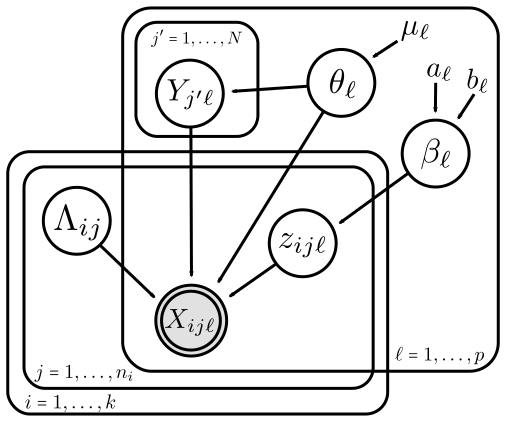
\includegraphics[width=0.5\textwidth]{finalFigures/recordLinkage_graphicalModel}
%\caption{Graphical representation of models \ref{model:cat}-\ref{model:string}.}
\label{fig:graphicalProcess}
\end{center}
\end{figure}


[\textbf{RCS}, Hall, Fienberg (2014, 2016); \textbf{RCS} (2015), Zanella, et al. (2016),
 \textbf{RCS} et al. (2017), (2018), Tancredi et al. (2019), Betancourt et al. (2020)]. 


}

\frame{

\begin{figure}[htbp]
\begin{center}
\includegraphics[scale=0.35]{finalFigures/latents_firstex}
%\caption{default}
%\label{default}
\end{center}
%\scriptsize{
%\begin{flushright}
%[Steorts, Hall, and Fienberg (2014), \emph{AIStats}.] \newline
%[Steorts, Hall, and Fienberg (2014), \emph{JASA}, In Revision.], [Steorts (2014), Submitted.] 
%\end{flushright}
%}
\end{figure}

}


\frame{

\begin{figure}[htbp]
\begin{center}
\includegraphics[scale=0.35]{finalFigures/latents_secondex}
%\caption{default}
%\label{default}
\end{center}
%\scriptsize{
%\begin{flushright}
%[Steorts, Hall, and Fienberg (2014), \emph{AIStats}.] \newline
%[Steorts, Hall, and Fienberg (2014), \emph{JASA}, In Revision], [Steorts (2014), Submitted.] 
%\end{flushright}
%}
\end{figure}

}

%\begin{frame}{Contemporary ER methods}
%  Past 20-30 years:
%  \begin{itemize}
%    \item more sophisticated Bayesian models
%    \item address limitations of Fellegi-Sunter method
%    \item poor scalability
%  \end{itemize}
%  
%  
%\end{frame}

\frame{
\frametitle{Our Goal}
\center
\Large
   Scaling Bayesian ER methods to millions of records without  sacrificing accuracy
   and crucially giving uncertainty of the ER task 

}

\frame{
\frametitle{Our Solution}
\center
\Large
   We propose a scalable joint (Bayesian) model for blocking and performing entity resolution, where the error from this joint task is exactly measured. 

}



\begin{frame}{Problem setup}
  \setlength{\leftmargini}{1.1em}
  \begin{columns}[onlytextwidth]
    \begin{column}{0.5\linewidth}
      Key assumptions:
      \begin{itemize}
        \item multiple tables\slash sources
        \item duplicates within and across tables
        \item attributes are aligned
        \item attributes are discrete
        \item some missing values
        \item no ground truth (unsupervised)
      \end{itemize}
    \end{column}
    \hfill
    \begin{column}{0.4\linewidth}
      \includegraphics[width=\linewidth]{multiple-datasets.pdf}
    \end{column}
  \end{columns}
  \pause
  \bigskip

  Output: approximate posterior distribution over the linkage structure
\end{frame}

\frame{
%\frametitle{Our contribution}

%Our solution relies on several key ingredients:
%\begin{enumerate}
%	\item Auxiliary variable representation of the model 
%	(superclusters) that removes dependencies between some 
%	of the variables (enables parallel computing)
%	\item Novel ``perturbation'' discrete sampling algorithm 
%	(used to update $Y$)
%	\item Sub-quadratic algorithm for updating the links between records 
%	and latent entities 
%	\item Collapsed Gibbs sampler (updates $Y$ and partition assignments)
%	\item Re-parametrization for string attributes in terms of a 
%	truncated string similarity function
%%	\item the Walker-Alias discrete sampling method (draw samples 
%%	from a non-uniform discrete distribution in constant 
%%	time)
%%	\item parallel\slash distributed computing
%\end{enumerate}
%Our key contributions include:

\begin{enumerate}
\item We propose a joint Bayesian model for blocking (latent entities) and entity resolution. 
\item We propose blocks (auxiliary partitions) that
induce conditional independencies between the latent entities. This enables distributed inference at the partition-level.
%, while crucially preserving the marginal posterior of the original model.
%\item Incorporating auxiliary partitions that
%induce conditional independencies between the entities. This enables distributed inference at the partition-level, while crucially preserving the marginal posterior of the original model. 
\item The blocking function (responsible for partitioning the entities) groups similar entities together while achieving well-balanced partitions.
\item Application of partially-collapsed Gibbs sampling in the context of distributed computing.
\item Improving computational efficiency:
\begin{enumerate}
\item[a)] Sub-quadratic algorithm for updating links based on indexing.
\item[b)] Truncation of the attribute similarities.
\item[c)] Perturbation sampling algorithm for updating the entity attributes, which relies on the Vose-Alias method.
\end{enumerate}
%	\item Auxiliary variable representation of the model 
%	(superclusters) that removes dependencies between some 
%	of the variables (enables parallel computing)
%	\item Novel ``perturbation'' discrete sampling algorithm 
%	(used to update $Y$)
%	\item Sub-quadratic algorithm for updating the links between records 
%	and latent entities 
%	\item Collapsed Gibbs sampler (updates $Y$ and partition assignments)
%	\item Re-parametrization for string attributes in terms of a 
%	truncated string similarity function
\end{enumerate}

Marchant, \textbf{RCS}, Kaplan, Rubinstein, and Elazar (2020).
}




\frame{
\frametitle{dblink}

\begin{figure}[htbp]
\begin{center}
\includegraphics[scale=0.6]{finalFigures/dblink}
%\caption{default}
%\label{default}
\end{center}
\end{figure}

}


%\section{Model}
%
%\begin{frame}{The \blink\ model}
%%  \setlength{\leftmargini}{1.1em}  
%%  Our work builds on the \blink\ model~(Steorts, 2015) for entity 
%%  resolution.
%%  \medskip
%
%
%  \begin{block}{Entities}
%    \begin{columns}[onlytextwidth]
%      \begin{column}{0.55\linewidth}
%        \begin{itemize}
%          \item Fixed population of entities $\mathcal{E} = \{1, \ldots, E\}$
%          \item Entity attribute $a$ has a finite domain with  
%          distribution $\phi_a$
%          \item Generate the value for attribute $a$ of entity $e$ by
%          
%          \[
%            y_{ea} \sim \operatorname{Discrete} \!\left( \phi_a \right) 
%          \]
%
%%          \item The value for attribute $a$ of entity $e$ is generated according 
%%          to
%%          \[
%%            y_{ea} \sim \operatorname{Discrete} \!\left( \phi_a \right) 
%%          \]
%        \end{itemize}
%      \end{column}
%      \hfill
%      \begin{column}{0.4\linewidth}
%        \includegraphics[width=.9\linewidth]{entities.pdf}
%      \end{column}
%    \end{columns}
%  \end{block}
%
%
%  \begin{block}{Linkage structure}
%    \begin{columns}[onlytextwidth]
%      \begin{column}{0.55\linewidth}
%        \begin{itemize}
%          \item Record $r$ in table $t$ is linked to an entity 
%          $\lambda_{tr} \in \mathcal{E}$ uniformly at random, viz.
%          \[
%            \lambda_{tr} \sim \operatorname{DiscreteUniform} \! \left( \mathcal{E} \right)
%          \]
%        \end{itemize}
%      \end{column}
%      \hfill
%      \begin{column}{0.4\linewidth}
%        \includegraphics[width=.9\linewidth]{linkage-structure.pdf}
%      \end{column}
%    \end{columns}
%  \end{block}  
%\end{frame}
%
%\begin{frame}[shrink=10]{The \blink\ model}
%  \setlength{\leftmargini}{1.1em}
%  \begin{block}{Distortion process}
%    \begin{columns}[onlytextwidth]
%      \begin{column}{0.55\linewidth}
%        \begin{itemize}
%          \item A distortion probability is associated with each attribute 
%          $a$ and table $t$
%          \[
%            \theta_{ta} \sim \operatorname{Beta} \! \left(\alpha_a, \beta_a \right)
%          \]
%          \item The value for attribute $a$ of record $r$ in table $t$ follows 
%          a hit-miss model
%            \begin{equation*}
%              \begin{split}
%                z_{tra} | \theta_{ta} &\sim \operatorname{Bernoulli} \! \left(\theta_{ta} \right) \\
%                x_{tra} | z_{tra}, y_{\lambda_{tr} a} &\sim 
%                  (1 - z_{tra}) \delta \! \left( y_{\lambda_{tr} a} \right) \\
%                   & \quad {} + z_{tra} \operatorname{Discrete} \! \left(\psi_a[y_{\lambda_{tr} a}] \right)
%              \end{split}
%            \end{equation*}
%          \item The distortion distribution may depend on a 
%          similarity function $\operatorname{sim}_a(\cdot, \cdot)$
%          \[
%            \psi_a[y](x) \propto \phi_a(x)  \exp \left( \operatorname{sim}_a(y, x) \right)
%          \]
%        \end{itemize}
%      \end{column}
%      \hfill
%      \begin{column}{0.4\linewidth}
%        \includegraphics[width=\linewidth]{distortion.pdf}
%      \end{column}
%    \end{columns}
%  \end{block}
%\end{frame}
%
%\begin{frame}{\dblink: a more general and scalable model}
%  \setlength{\leftmargini}{1.1em}
%  We propose a distributed version of \blink\ called \alert{\dblink}
%  
%  $\hookrightarrow$ distributed, more general model, faster inference 
%  algorithms
%  \pause
%  \bigskip
%
%
%  \begin{block}{Modelling differences in \dblink}
%    \begin{itemize}
%      \item Supports missing record values (MCAR)
%      \item Supports arbitrary attribute similarity functions (one for each 
%      attribute)
%      \item Incorporates a kind of ``blocking'': auxiliary partitions
%    \end{itemize}
%  \end{block}
%\end{frame}
%
%\begin{frame}{Auxiliary partitions}
%  \setlength{\leftmargini}{1.1em}
%  \begin{columns}[onlytextwidth]
%    \begin{column}{0.55\linewidth}
%      \begin{itemize}
%        \item Enables distributed inference
%        \item Crucially leaves the marginal posterior \alert{unchanged}
%        \item Partition the space of entities 
%        $\mathcal{V}_\otimes = \bigotimes_a \mathcal{V}_a$ using a 
%        deterministic function $\texttt{PartFn}: \mathcal{V}_\otimes \to 
%        \{1,\ldots, P\}$
%        \item Update the model: now record $r$ in table $t$ is assigned to 
%        a partition $\gamma_{tr}$, then to an entity $\lambda_{tr}$ 
%        within the partition
%        \begin{equation*}
%          \begin{split}
%            \gamma_{tr} | \mathbf{Y} &\sim \operatorname{Discrete} \! 
%              \left(\frac{|\mathcal{E}_1|}{|\mathcal{E}|}, \ldots, \frac{|\mathcal{E}_P|}{|\mathcal{E}|} \right) \\
%            \lambda_{tr} | \gamma_{tr} &\sim \operatorname{DiscreteUniform} \! \left( \mathcal{E}_{\gamma_{tr}}\right)
%          \end{split}
%        \end{equation*}
%      \end{itemize}
%    \end{column}
%    \begin{column}{0.38\linewidth}
%      \includegraphics[width=\linewidth]{entity-partition.pdf}
%    \end{column}
%  \end{columns}
%\end{frame}


\section{Inference}
\begin{frame}{Distributed Markov chain Monte Carlo}
  Since the posterior for the linkage structure $p(\Lambda | X)$ is not 
  tractable, we resort to \alert{approximate inference}.
  \vspace*{1em}
  \pause

  We propose an MCMC algorithm based on the \alert{partially-collapsed Gibbs} 
  framework~(van Dyk and Park, 2008):
  \begin{itemize}
    \item regular Gibbs updates for the distortion probabilities $\theta_{ta}$, 
    distortion indicators $z_{tra}$ and links $\lambda_{tr}$
    \item ``marginalization'' and ``trimming'' are applied to jointly update 
    the entity attributes $y_{ea}$ and the partition assignments for the 
    linked records
    \item order of the updates is important (to preserve the stationary 
    distribution)
  \end{itemize}
\end{frame}

\begin{frame}{Distributed Markov chain Monte Carlo}
%  \begin{itemize}
%    \item Distribute inference using a master-worker architecture
%    \item Possible since records\slash entities are conditionally independent 
%    across partitions
%  \end{itemize}
  
  \begin{center}
    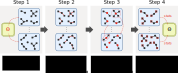
\includegraphics[width=\linewidth]{./figures/distributed-transition-operator.pdf}
  \end{center}
\end{frame}


\begin{frame}{Tricks for speeding up inference}
  Two main bottlenecks:
  \begin{enumerate}
    \item linkage structure update 
    $\mathcal{O}(\text{\# records} \times \text{\# entities})$ 
    \item entity attribute update 
    $\mathcal{O}(\text{\# entities} \times \text{domain size})$   \end{enumerate}
  
   \vspace*{2em}
   
  \pause
   Solutions:
   \begin{enumerate}
      \item Indexing: Maintain indices from ``entity attributes $\to$ entities'' and 
      ``entities $\to$ linked records." This allows us to prune candidate links for a record
   \item Thresholding similarity scores
    \item Express the distribution for the entity attribute update as a 
      two-component perturbation mixture model
   \end{enumerate}
   \end{frame}


%  \begin{block}{Thresholding similarity scores}
%    \begin{itemize}
%      \item Helps with both bottlenecks
%      \item Similarities below a specified cut-off are set to zero
%      \item A higher cut-off is less accurate, but more efficient
%    \end{itemize}
%  \end{block}
%  \pause

%  \begin{block}{Indexing}
%    \begin{itemize}
%      \item Addresses bottleneck~1
%      \item Maintain indices from ``entity attributes $\to$ entities'' and 
%      ``entities $\to$ linked records''
%      \item Can then efficiently prune the set of candidate links for a 
%      record
%      \item Express the distribution for the entity attribute update as a 
%      two-component perturbation mixture model
%    \end{itemize}
%  \end{block}
%\end{frame}

%\begin{frame}[shrink=7]{Tricks for speeding up inference}
%
%%  \bigskip
%%  \begin{block}{Perturbation sampling}
%%    \begin{itemize}
%%      \item Addresses bottleneck~2
%%      \item Express the distribution for the entity attribute update as a 
%%      two-component mixture
%%      \[
%%        p(y_a|\omega) = w_\mathrm{base} q_\mathrm{base}(y_a) + w_\mathrm{pert} q_\mathrm{pert}(y_a|\omega)
%%        \]
%%      \item $q_\mathrm{pert}$ generally has a much larger weight and a much 
%%      smaller support (faster to sample from)
%%      \item Important for large domains
%%    \end{itemize}
%%  \end{block}
%\end{frame}



\frame{
\frametitle{Experiments}

\begin{itemize}
  \item \texttt{ABSEmployee}. A synthetic data set used 
  internally for linkage experiments by the ABS.
%  It simulates an employment census and two supplementary 
%  surveys. 
  \item \texttt{NCVR}. Two snapshots from the North Carolina 
  Voter Registration database taken two months 
  apart. 
%  The snapshots are filtered to include only those voters 
%  whose details changed over the two-month period.
%  We use the full name, age, gender and zip code attributes.
  \item \texttt{NLTCS}. A subset of the National Long-Term 
  Care Survey comprising the 
  1982, 1989 and 1994 waves.
  %\footnote{A subset must be used as race was 
  %subsampled in the other three years, making it unsuitable for ER.}
  % NM-1: Removing this footnote purely to fix the layout.
  % RS: Okay. 
%  We use the SEX, DOB, STATE and REGOFF attributes.
  \item \texttt{SHIW0810}. A subset from the Bank of Italy's 
  Survey on Household Income and Wealth
  comprising the 2008 and 2010 waves.
  %\footnote{Available at \url{http://github.com/[REDACTED]}} 
%    We use 8 attributes: IREG, SESSO, ANASC, STUDIO, PAR, 
%  STACIV, PERC and CFDIC.
  % NM-1: The SHIW data set we used is _different_ to the one 
  % that appears in the italy R package.
  % The version we used is based on the raw data from the 
  % Bank of Italy website, with a correction to the NORD 
  % variable (done using an R script that I wrote).
  % I guess we could make this available on GitHub...
  % RS-1: Thanks for clarifying. Would be helpful to put on Github since they are different and there could be confusion with the two different versions. 
  
  \item \texttt{RLdata10000}. A synthetic data set provided 
  with the \texttt{RecordLinkage} R 
  package. % because all attributes are missing.
  % NM-1: This is not true. There are "non-missing" values 
  % in fname_c2 and lname_c2 for RLdata10000 
  % (you might be thinking of RLdata500?).
  % RS-1: Yes. Thank you, NM! 
\end{itemize}

}







\begin{frame}{Experiments}
  \begin{itemize}
    \item Implemented \dblink\ and baselines in Apache Spark
    \item Ran experiments on a local server and Amazon EMR
    \item (Mostly) used a sample size of $10^3$ after burnin (of 
    $10^3$ iterations) and thinning (keeping every 10th iteration)
    \item 3 real and 2 synthetic data sets
  \end{itemize}
  \pause

  \begin{center}
    \footnotesize
    \begin{tabularx}{\linewidth}{l *{3}{c} *{2}{Y}}
      \toprule
      Data set & \# records & \# tables & \# entities & 
      \multicolumn{2}{c}{\# attributes} \\ 
      \cmidrule{5-6}
      & & & & {\footnotesize categorical} & {\footnotesize string } \\
      \midrule
      $\star$ \texttt{ABSEmployee} & 600,000 & 3 & 400,000 & 4 & 0 \\
      \texttt{NCVR}        & 448,134 & 2 & 296,433 & 3 & 3 \\
      \texttt{NLTCS}       &  57,077 & 3 &  34,945 & 6 & 0 \\
      \texttt{SHIW0810}    &  39,743 & 2 &  28,584 & 8 & 0 \\
      $\star$ \texttt{RLdata10000} &  10,000 & 1 &   9,000 & 2 & 3 \\
      \bottomrule
    \end{tabularx}
  \end{center}
\end{frame}

\frame{



\scriptsize{
\begin{table}
	\centering
	\caption{Assessment of the pairwise linkage performance for dblink and FS method as our baseline. We note that FS is supervised and does not propagate the entity resolution error exactly compared to dblink.\footnote{Comparisons to other semi-supervised methods are the same.}}
	\vspace*{1em}
	\begin{tabular}{l l *{3}{c}}
		\toprule
		Data set    & Method & \multicolumn{3}{c}{Pairwise measure} \\
		\cmidrule(){3-5}
		 & & Precision & Recall & F1-score \\
		\midrule
		\multirow{2}{*}{\texttt{ABSEmployee}} 
		 & dblink                  & \textbf{0.9943} & \textbf{0.8867} & \textbf{0.9374} \\
		 & Fellegi-Sunter (100)  & {0.9964} & {0.9510} & {0.9736} \\
		 & Fellegi-Sunter (10)  & {0.4321} & {0.6034} & {0.9736} \\

		 
%		 & Near matching         & 0.0543 & \textbf{0.9970} & 0.1030 \\
%		 & Exact matching        & \textbf{0.9964} & 0.8849 & 0.9374 \\
		\midrule
		\multirow{2}{*}{\texttt{NCVR}}
		 & dblink                 & \textbf{0.9179} & \textbf{0.9654} & \textbf{0.9411} \\
		 & Fellegi-Sunter (100)  & 0.8989 & {0.9974} & {0.9456} \\
		 & Fellegi-Sunter (10)  & 0.8989 & {0.9974} & {0.9456} \\
%		 & Near matching         & 0.9899 & 0.7443 & 0.8497 \\
%		 & Exact matching        & \textbf{0.9925} & 0.0017 & 0.0034 \\
		\midrule
		\multirow{2}{*}{\texttt{NLTCS}}
		 & dblink                  & \textbf{0.8363} &  \textbf{0.9102} &  \textbf{0.8717} \\
		 & Fellegi-Sunter (100)  & 0.7969 & {0.9959} & {0.8853} \\
		  & Fellegi-Sunter (10)  & 0.1902 & {0.9999} & {0.3196} \\
%		 & Near matching         & 0.0385 & 0.9656 & 0.0740 \\
%		 & Exact matching        & \textbf{0.8451} & 0.9234 & 0.8825 \\ 
		\bottomrule
	\end{tabular}
\end{table}
}
}


%\frame{
%
%
%
%\scriptsize{
%\begin{table}
%	\centering
%	\caption{Assessment of the pairwise linkage performance for dblink and FS method as our baseline. We note that FS is supervised and does not propagate the entity resolution error exactly compared to dblink. }
%	\begin{tabular}{l l *{3}{c}}
%		\toprule
%		Data set    & Method & \multicolumn{3}{c}{Pairwise measure} \\
%		\cmidrule(){3-5}
%		 & & Precision & Recall & F1-score \\
%		\midrule
%		\multirow{2}{*}{\texttt{ABSEmployee}} 
%		 & dblink                  & \textbf{0.9943} & \textbf{0.8867} & \textbf{0.9374} \\
%		 & Fellegi-Sunter (100)  & {0.9964} & {0.9510} & {0.9736} \\
%		 & Fellegi-Sunter (10)  & {0.4321} & {0.6034} & {0.9736} \\
%
%		 
%%		 & Near matching         & 0.0543 & \textbf{0.9970} & 0.1030 \\
%%		 & Exact matching        & \textbf{0.9964} & 0.8849 & 0.9374 \\
%		\midrule
%		\multirow{2}{*}{\texttt{NCVR}}
%		 & dblink                 & \textbf{0.9179} & \textbf{0.9654} & \textbf{0.9411} \\
%		 & Fellegi-Sunter (100)  & 0.8989 & {0.9974} & {0.9456} \\
%		 & Fellegi-Sunter (10)  & 0.8989 & {0.9974} & {0.9456} \\
%%		 & Near matching         & 0.9899 & 0.7443 & 0.8497 \\
%%		 & Exact matching        & \textbf{0.9925} & 0.0017 & 0.0034 \\
%		\midrule
%		\multirow{2}{*}{\texttt{NLTCS}}
%		 & dblink                  & \textbf{0.8363} &  \textbf{0.9102} &  \textbf{0.8717} \\
%		 & Fellegi-Sunter (100)  & 0.7969 & {0.9959} & {0.8853} \\
%		  & Fellegi-Sunter (10)  & 0.1902 & {0.9999} & {0.3196} \\
%%		 & Near matching         & 0.0385 & 0.9656 & 0.0740 \\
%%		 & Exact matching        & \textbf{0.8451} & 0.9234 & 0.8825 \\ 
%		\midrule
%		\multirow{2}{*}{\texttt{SHIW0810}}
%		 & dblink                  & \textbf{0.2529} & \textbf{0.5378} & \textbf{0.3440} \\
%		 & Fellegi-Sunter (100)  & 0.1263 & {0.8480} & 0.2198 \\
%		& Fellegi-Sunter (10)  & 0.0947 & {0.9244} & 0.1719 \\
%%		 & Near matching         & 0.0043 & \textbf{0.9111} & 0.0086 \\
%%		 & Exact matching        & 0.1263 & 0.7608 & 0.2166 \\ 
%		\midrule
%		\multirow{2}{*}{\texttt{RLdata10000}}
%		 & dblink                  & \textbf{0.6310} & \textbf{0.9970} & \textbf{0.7729} \\
%		 & Fellegi-Sunter (100)  & {0.9153} & {0.9940} & {0.9530} \\
%		 & Fellegi-Sunter (10)  & 0.1706 & {1.0000} & 0.2915 \\
%%		 & Near matching         & 0.9176 & 0.9690 & 0.9426 \\
%%		 & Exact matching        & \textbf{1.0000} & 0.0080 & 0.0159 \\ 
%		\bottomrule
%	\end{tabular}
%\end{table}
%}
%}

\frame{
\frametitle{Posterior Bias Plot}

\begin{figure}[htbp]
\begin{center}
\includegraphics[scale=1]{figures/posterior-bias-plot}
\caption{Error in the posterior and prior estimates for the number of observed entities for d-blink. The results show that the posterior estimate is very sharp and typically underestimates the true number, which is consistent with \textbf{RCS}, Hall, Fienberg (2016). }
\label{default}
\end{center}
\end{figure}


}

\begin{frame}{Convergence of \dblink\ versus \blink}
  We examined the rate of convergence of \dblink\ versus \blink\ 
  on \texttt{RLdata10000} without partitioning.
  
  \begin{center}
    \includegraphics[height=0.45\textheight]{figures/convergence-num-ent-blink-dblink.pdf}
    \hfill
    \includegraphics[height=0.45\textheight]{figures/convergence-agg-dist-blink-dblink.pdf}
  \end{center}

  \texttt{d-blink} converges rapidly, however \blink\ fails to reach 
  the equilibrium distribution within 11 hours.
\end{frame}


%\section{Conclusions}
%\begin{frame}{Conclusions}
%  \begin{block}{Summary}
%    \begin{itemize}
%      \item Achieve a significant speed-up: roughly by a factor of $300 \times$
%      \item Promising for linking moderate-sized data sets ($\sim 10^6$ records)
%      \item Competitive linkage quality on the data sets tested
%    \end{itemize}  
%  \end{block}
%  \pause
%  \bigskip 
%
%  \begin{block}{Future work}
%    \begin{itemize}
%      \item Microclustering priors
%      \item Ability to incorporate some labelled data (semi-supervised)
%      \item Integration with downstream tasks
%    \end{itemize}
%  \end{block}
%\end{frame}

\frame{
\frametitle{Ongoing work}

\begin{enumerate}
\item Developing a general set of Bayesian ER models that are non-parametric and allow for more automated tuning of 
any parameters. 
\item Allowing this model to be flexible to names that are not English (Hispanic, Arabic, etc). 
\item Developing a parallelized algorithm for this model. 
\item Integration of this into d-blink, which is quite extensive. 
\item Pushing the limits of scalability. 
\item Models for structured and unstructured databases in an unsupervised manner. 
\end{enumerate}

}

\frame{
\center
Questions?\\
Contact: beka@stat.duke.edu\\
\vspace*{1em}
This work has been supported by NSF CAREER and the Sloan Foundation, and the ideas of this paper are of the authors and not of the granting organization.  \\

\vspace*{1em}
\url{https://github.com/resteorts/record-linkage-tutorial} \\
\url{https://arxiv.org/abs/1909.06039} \\
\url{https://github.com/cleanzr/dblink}

}


%\appendix
%
%\begin{frame}{Does partitioning result in efficiency gains?}
%  \begin{itemize}
%    \item Measure efficiency using \alert{ESS rate}---the effective sample 
%    size generated per unit time
%    \item \alert{Speed-up factor} is the ESS rate relative to a baseline 
%    without partitioning
%    \item Observe a near-linear speed-up for the \texttt{NLTCS} data set
%    (tapering off beyond $\sim 20$ partitions)    
%  \end{itemize}
%
%  \begin{center}
%    \includegraphics[width=0.9\textwidth]{figures/plot-partitions-speed-up-muppet.pdf}
%  \end{center}
%\end{frame}
%
%
%\section{Model}
%
%\begin{frame}{The \blink\ model}
%%  \setlength{\leftmargini}{1.1em}  
%%  Our work builds on the \blink\ model~(Steorts, 2015) for entity 
%%  resolution.
%%  \medskip
%
%
%  \begin{block}{Entities}
%    \begin{columns}[onlytextwidth]
%      \begin{column}{0.55\linewidth}
%        \begin{itemize}
%          \item Fixed population of entities $\mathcal{E} = \{1, \ldots, E\}$
%          \item Entity attribute $a$ has a finite domain with  
%          distribution $\phi_a$
%          \item Generate the value for attribute $a$ of entity $e$ by
%          
%          \[
%            y_{ea} \sim \operatorname{Discrete} \!\left( \phi_a \right) 
%          \]
%
%%          \item The value for attribute $a$ of entity $e$ is generated according 
%%          to
%%          \[
%%            y_{ea} \sim \operatorname{Discrete} \!\left( \phi_a \right) 
%%          \]
%        \end{itemize}
%      \end{column}
%      \hfill
%      \begin{column}{0.4\linewidth}
%        \includegraphics[width=.9\linewidth]{entities.pdf}
%      \end{column}
%    \end{columns}
%  \end{block}
%
%
%  \begin{block}{Linkage structure}
%    \begin{columns}[onlytextwidth]
%      \begin{column}{0.55\linewidth}
%        \begin{itemize}
%          \item Record $r$ in table $t$ is linked to an entity 
%          $\lambda_{tr} \in \mathcal{E}$ uniformly at random, viz.
%          \[
%            \lambda_{tr} \sim \operatorname{DiscreteUniform} \! \left( \mathcal{E} \right)
%          \]
%        \end{itemize}
%      \end{column}
%      \hfill
%      \begin{column}{0.4\linewidth}
%        \includegraphics[width=.9\linewidth]{linkage-structure.pdf}
%      \end{column}
%    \end{columns}
%  \end{block}  
%\end{frame}
%
%\begin{frame}[shrink=10]{The \blink\ model}
%  \setlength{\leftmargini}{1.1em}
%  \begin{block}{Distortion process}
%    \begin{columns}[onlytextwidth]
%      \begin{column}{0.55\linewidth}
%        \begin{itemize}
%          \item A distortion probability is associated with each attribute 
%          $a$ and table $t$
%          \[
%            \theta_{ta} \sim \operatorname{Beta} \! \left(\alpha_a, \beta_a \right)
%          \]
%          \item The value for attribute $a$ of record $r$ in table $t$ follows 
%          a hit-miss model
%            \begin{equation*}
%              \begin{split}
%                z_{tra} | \theta_{ta} &\sim \operatorname{Bernoulli} \! \left(\theta_{ta} \right) \\
%                x_{tra} | z_{tra}, y_{\lambda_{tr} a} &\sim 
%                  (1 - z_{tra}) \delta \! \left( y_{\lambda_{tr} a} \right) \\
%                   & \quad {} + z_{tra} \operatorname{Discrete} \! \left(\psi_a[y_{\lambda_{tr} a}] \right)
%              \end{split}
%            \end{equation*}
%          \item The distortion distribution may depend on a 
%          similarity function $\operatorname{sim}_a(\cdot, \cdot)$
%          \[
%            \psi_a[y](x) \propto \phi_a(x)  \exp \left( \operatorname{sim}_a(y, x) \right)
%          \]
%        \end{itemize}
%      \end{column}
%      \hfill
%      \begin{column}{0.4\linewidth}
%        \includegraphics[width=\linewidth]{distortion.pdf}
%      \end{column}
%    \end{columns}
%  \end{block}
%\end{frame}
%
%\begin{frame}{\dblink: a more general and scalable model}
%  \setlength{\leftmargini}{1.1em}
%  We propose a distributed version of \blink\ called \alert{\dblink}
%  
%  $\hookrightarrow$ distributed, more general model, faster inference 
%  algorithms
%  \pause
%  \bigskip
%
%
%  \begin{block}{Modelling differences in \dblink}
%    \begin{itemize}
%      \item Supports missing record values (MCAR)
%      \item Supports arbitrary attribute similarity functions (one for each 
%      attribute)
%      \item Incorporates a kind of ``blocking'': auxiliary partitions
%    \end{itemize}
%  \end{block}
%\end{frame}
%
%\begin{frame}{Auxiliary partitions}
%  \setlength{\leftmargini}{1.1em}
%  \begin{columns}[onlytextwidth]
%    \begin{column}{0.55\linewidth}
%      \begin{itemize}
%        \item Enables distributed inference
%        \item Crucially leaves the marginal posterior \alert{unchanged}
%        \item Partition the space of entities 
%        $\mathcal{V}_\otimes = \bigotimes_a \mathcal{V}_a$ using a 
%        deterministic function $\texttt{PartFn}: \mathcal{V}_\otimes \to 
%        \{1,\ldots, P\}$
%        \item Update the model: now record $r$ in table $t$ is assigned to 
%        a partition $\gamma_{tr}$, then to an entity $\lambda_{tr}$ 
%        within the partition
%        \begin{equation*}
%          \begin{split}
%            \gamma_{tr} | \mathbf{Y} &\sim \operatorname{Discrete} \! 
%              \left(\frac{|\mathcal{E}_1|}{|\mathcal{E}|}, \ldots, \frac{|\mathcal{E}_P|}{|\mathcal{E}|} \right) \\
%            \lambda_{tr} | \gamma_{tr} &\sim \operatorname{DiscreteUniform} \! \left( \mathcal{E}_{\gamma_{tr}}\right)
%          \end{split}
%        \end{equation*}
%      \end{itemize}
%    \end{column}
%    \begin{column}{0.38\linewidth}
%      \includegraphics[width=\linewidth]{entity-partition.pdf}
%    \end{column}
%  \end{columns}
%\end{frame}
%
%
%\begin{frame}[shrink=7]{Partition function}
%  \begin{block}{Desirable properties}
%    \begin{itemize}
%      \item \emph{Balanced:} each part has equal probability mass under the 
%      distribution over $\mathcal{V}_\otimes$
%      \item \emph{Good separation:} high similarity within a part, low 
%      similarity between parts
%    \end{itemize}
%  \end{block}
%
%  \begin{block}{k-d tree partition function}
%    \begin{columns}[onlytextwidth]
%      \begin{column}{0.55\linewidth}
%        \begin{itemize}
%          \item Recursively partitions $\mathcal{V}_\otimes$
%          \item Each node is associated with a binary splitting rule on one of 
%          the attributes 
%          \item Use the empirical distribution from the tables to approximate 
%          the distribution over $\mathcal{V}_\otimes$
%        \end{itemize}
%      \end{column}
%      \begin{column}{0.4\linewidth}
%        \includegraphics[width=\linewidth]{kd-tree.pdf}
%      \end{column}
%    \end{columns}
%  \end{block}
%\end{frame}
%
%\begin{frame}{What about load balancing?}
%  \begin{itemize}
%    \item Measure the \alert{relative absolute deviation} from the 
%    perfectly-balanced configuration along the Markov chain
%    \item Results indicate that the $k$-d tree partition function results 
%    in good load balancing
%  \end{itemize}
%
%  \begin{center}
%    \includegraphics[width=0.9\textwidth]{partition-sizes-plot.pdf}
%  \end{center}
%\end{frame}
%
%\begin{frame}{Linkage quality}
%  \begin{center}
%    \scriptsize
%    \begin{tabular}{l l *{3}{c}}
%      \toprule
%      Data set    & Method & Precision & Recall & F1-score \\
%      %\cmidrule(lr){3-5} 
%      \midrule
%      \multirow{4}{*}{\texttt{ABSEmployee}} 
%      & \dblink\              & 0.9763 & \textbf{0.8530} & \textbf{0.9105} \\
%      & Fellegi-Sunter (10)   & \textbf{0.9963} & 0.8346 & 0.9083 \\
%      & Fellegi-Sunter (100)  & \textbf{0.9963} & 0.8346 & 0.9083 \\
%      & Exact Matching        & 0.9939 & 0.8346 & 0.9074 \\
%      \midrule
%      \multirow{4}{*}{\texttt{NCVR}}
%      & \dblink\              & 0.9145 & \textbf{0.9653} & \textbf{0.9392} \\
%      & Fellegi-Sunter (10)   & 0.9868 & 0.7874 & 0.9083 \\
%      & Fellegi-Sunter (100)  & 0.9868 & 0.7874 & 0.9083 \\
%      & Exact Matching        & \textbf{0.9925} & 0.0017 & 0.0034 \\
%      \midrule
%      \multirow{4}{*}{\texttt{NLTCS}}
%      & \dblink\              & 0.8319 & \textbf{0.9103} & 0.8693 \\
%      & Fellegi-Sunter (10)   & \textbf{0.9094} & 0.9087 & \textbf{0.9090} \\
%      & Fellegi-Sunter (100)  & \textbf{0.9094} & 0.9087 & \textbf{0.9090} \\
%      & Exact Matching        & 0.8995 & 0.9087 & 0.9040 \\ 
%      \midrule
%      \multirow{4}{*}{\texttt{SHIW0810}}
%      & \dblink\              & \textbf{0.2514} & 0.5396 & \textbf{0.3430} \\
%      & Fellegi-Sunter (10)   & 0.0028 & 0.9050 & 0.0056 \\
%      & Fellegi-Sunter (100)  & 0.0025 & \textbf{0.9161} & 0.0050 \\
%      & Exact Matching        & 0.1263 & 0.7608 & 0.2166 \\ 
%      \midrule
%      \multirow{4}{*}{\texttt{RLdata10000}}
%      & \dblink\              & 0.6334 & \textbf{0.9970} & 0.7747 \\
%      & Fellegi-Sunter (10)   & 0.9957 & 0.6174 & 0.7622 \\
%      & Fellegi-Sunter (100)  & 0.9364 & 0.8734 & \textbf{0.9038} \\
%      & Exact Matching        & \textbf{1.0000} & 0.0080 & 0.0159 \\ 
%      \bottomrule
%    \end{tabular}
%  \end{center}
%\end{frame}
%
%
%\begin{frame}[shrink=10]{Behavior of the prior}
%  \setlength{\leftmargini}{1.1em}
%  \vspace{2cm}
%  \begin{columns}
%    \begin{column}{0.53\linewidth}
%      \begin{itemize}
%        \item The prior we use on the entities\slash links is termed a 
%        \emph{coupon-collecting prior} in the literature~(Pitman, 2006)
%        \item Sensitive to the size of the population $E = |\mathcal{E}|$
%        \item Strongly informative for the number of entities present in 
%        the data
%        \item Alternatives: a Pitman-Yor Process or microclustering 
%        priors
%      \end{itemize}
%    \end{column}
%    \hfill
%    \begin{column}{0.45\linewidth}
%      \includegraphics[width=\linewidth]{coupon-collecting.png}
%    \end{column}
%  \end{columns}
%\end{frame}
%
%\frame{
%\frametitle{Microclustering}
%
%The above work led to discovery that many clustering algorithms for Bayesian non-parametrics are inappropriate for entity resolution. 
%\pause
%
%\vspace*{1em}
%
%The cluster sizes grow sub-linearly with the number of records.
%
%\pause
%\vskip 1em
%A sequence of random partitions $(C_N
%: N=1, 2, \ldots)$ exhibits the \emph{microclustering property} if $M_N$ is
%$o_p(N)$, where $M_N$ is the size of the largest cluster in
%$C_N$. 
%%Equivalently, $M_N \,/\, N \rightarrow 0$ in probability as $N
%%\rightarrow \infty$.
%
%\pause
%\vskip 1em
%A clustering model exhibits the microclustering property if $(C_N
%: N=1, 2, \ldots)$  implied by that model satisfies the above definition.
%
%\vskip 1em
%
%
%[Zanella, Betancourt, Wallach, Miller, Zaidi, and \textbf{RCS} (2016), Zanella, Betancourt, \textbf{RCS} (2019), Submitted]\\
%NSF CAREER Award 2017
%}

%\frame{
%\frametitle{Theoretical Limits for  Entity Resolution}
%Are there theoretical limits for entity resolution? Yes! 
%
%\vspace*{1em}
%
%Two very different approaches:
%
%\begin{enumerate}
%\item Johndrow, Lum, and Dunson, Biometrika, 2018.
%\begin{itemize}
%\item The authors show that that for $p$ features or when the number of entities is small compared to the number of records that entity resolution is ``effectively impossible." 
%\end{itemize}
%\item \textbf{RCS}, Barnes, Neiswanger (2017), AIStats, \url{http://proceedings.mlr.press/v54/}.
%\begin{itemize}
%\item We derive performance bounds (lower bounds) using the KL divergence on when a latent entity is mis-classified, showing when the bounds are tight.
%\end{itemize}
%\end{enumerate} 
%
%%\begin{itemize}
%%\item The first paper sheds light on the implausibility of entity resolution. The second paper sheds light on the plausibility and implausibility of entity resolution. 
%
%%\item Goal: Derive a lower bound for the probability that the linkage structure is mis-classified. 
%%\end{itemize}
%}
%
%\frame{
%\Large
%\center
%How could we apply this to a real problem with little or no training data?\\
%\vspace*{1em}
%What types of problems might we encounter?
%}
%
%\frame{
%\frametitle{El Salvadoran Conflict}
%
%\begin{itemize}
%\item El Salvador underwent a civil war from 1980 to 1991.
%\item The United Nations created a Truth Commission (UNTC) to record death casualties/disappearances related to the war by inviting witnesses through newspaper, radio, and television advertisements.
%\item Human rights groups often depend on accurate estimates and evaluations of the number of documented identifiable deaths for purposes of court ruling, etc. 
%\end{itemize}
%\begin{figure}
%\center
%\includegraphics[width=0.7\textwidth]{finalFigures/department}
%\end{figure}
%}
%
%
%\frame{
%\frametitle{UNTC dataset}
%
%\begin{figure}
%\center
%\includegraphics[width=1\textwidth]{finalFigures/data-snapshot.png}
%\end{figure}
%
%\vspace*{4em}
%
%We utilize a similar type of framework to Marchant et. al (2019), however we consider a set of more flexible priors on the linkage structure and a different type of string metrics for the hispanic names. 
%}
%
%\frame{
%\frametitle{Experiments on UNTC Data}
%\begin{itemize}
%\item We consider the following attributes: first name, family name, date of death (year, month, day), and location of death (department, municipality). 
%\item Given that we do not know the true number of latent entities in departments 1 or 7, we will assume that the number are close to the size calculated from the hand matched labels, which is 680 unique entities in total.
%\end{itemize}
%}
%
%
%\frame{
%\frametitle{Parameter Setting}
%DP clustering prior currently gives the best result in terms of precision (0.8) and recall (0.8), with hyperparameter settings $(a,b)=(1, 99)$ and $\vartheta = 2$.
%\begin{table}[h]
%\center
%\caption{\textbf{DP prior}: Best configuration of attribute similarity measures for \texttt{UNTC} data set. Recall that similarities below $S_{cut}$ are effectively treated as zero (truncation) in order to speed up the sampling. }
%\label{tbl:sv-dp-best}
%\begin{tabular}{*{3}{c}}
%\toprule
%Field & $S_{max}$ & $S_{cut}$ \\
%\midrule
%firstname & 40 & 28 \\
%lastname & 40 & 28 \\
%dept & 20 & 10 \\
%muni & 20 & 10 \\
%day & 10 & 5 \\
%month & 10 & 5 \\
%year & 20 & 10 \\
%\bottomrule
%\end{tabular}
%\end{table}
%}
%
%
%\frame{
%\frametitle{Results}
%\begin{figure}[h]
%\center
%\includegraphics[width=0.6\textwidth]{newfigs/0305-pop-hist.pdf}
%\caption{\label{fig:sv-trace-dp} \textbf{DP prior on UNTC:} Posterior density plot of the number of distinct entities from the Gibbs samples, along with the posterior mean of 680.66 (black line), ``true" value of 680 (red line) and 95\% credible interval of [677, 684] (blue dashed line).}
%\end{figure} 
%}
%
%\frame{
%\frametitle{Results}
%\begin{table}[h]
%\center
%\tiny
%\caption{Comparison of PYP, DP and Uniform prior on UNTC.}
%\begin{tabular}{*{11}{c}}
%\toprule
%Prior & $a$ & $b$ & $\vartheta$ & $\sigma$ & Precision & Recall & Posterior mean & SE & Runtime (sec) \\
%\midrule
%\multirow{3}{*}{PYP} & \multirow{3}{*}{1} & \multirow{3}{*}{99} 
%&1.7272 & 0.9890 & \textbf{0.900} & 0.153 & 725.45 & 1.27 & 892.17 \\
%& & & 2.5663 & 0.9885 & 0.900 & 0.153 & 725.58 & 1.64 & 894.91 \\
%& & & 4.6017 & 0.9875 & 0.900 & 0.153 & 728.21 & 1.27 & 803.36  \\
% \midrule
%\multirow{3}{*}{DP} & \multirow{3}{*}{1} & \multirow{3}{*}{99}
% & 1 & - & 0.770 & 0.797 & 678.237 & 1.38 & 997.8 \\
% & & & 2 & - & \textbf{0.797} & \textbf{0.797} & 680.08 & 1.79 & 1054.2 \\
% & & & 3 & - & 0.793 & 0.780 & 682.18 & 1.74 & 1042.2 \\
% \midrule
% \multirow{2}{*}{Uniform}
%& 1 & 73.5 & - & - & \textbf{0.867} & 0.661 & 692.47 & 2.58 & 3490.09 \\
%& 1 & 99 & - & - & 0.826 & 0.644 & 688.84 & 2.18 & 3280.19 \\
%\bottomrule
%\end{tabular}
%\end{table}
%}
%
%%\frame{
%%\frametitle{Discussion on UNTC Experiments}
%%\begin{itemize}
%%\item So far the DP prior is able to generate the best results in terms of balanced precision and recall.
%%\item The PYP and Uniform prior consistently overestimate the true number of entities.
%%\item The uniform prior is the slowest to mix. Because the DP and PYP prior are more subjective and flexible than the Uniform prior, mixing of the Gibbs sampler is faster.
%%\end{itemize}
%%}
%
%\frame{
%\frametitle{Example of False Positive Error}
%\begin{table}[h]
%\center
%\tiny
%\caption{Our model currently clusters these records to the same latent entity. But according to the hand matched labels, there are actually two latent entities here. We believe that this hand-matched label could be easily labeled as match or not-match depending on the hand-matcher. }
%\begin{tabular}{*{7}{c}}
%\toprule
%Firstname & Lastname & Year & Month & Day & Department & Municipality  \\
%\midrule
%CARMEN & ALFARO  & 1982 & 3 & 21 & 7 & 716 \\
%JOSE       & ALFARO GAMES & 1980 & 3 & 22 & 7 & 716 \\
%CARMEN & ALFARO GAMES & 1980 & 3 & 22 & 7 & 716 \\
%\bottomrule
%\end{tabular}
%\end{table}
%
%%\vspace{0.5em}
%%\textcolor{red}{ }
%}
%













\end{document}
